% !TEX root = ../main.tex

\section{Methods}
\label{sec:data}

\subsection{Simulated data}

In order to compare the two methods while controlling for their correct performance, we simulated a 400 seconds (TR = 2 s) activity-inducing signal with five neuronal events, convolved it with the canonical HRF, and we added noise of different sources (physiological, thermal, and motion-related) with different signal-to-noise ratios (SNR = [20 dB, 10 dB, 3 dB]) that represent low, medium and high levels of noise as shown in Figure~\ref{fig:sim_and_hrf}A. Noise was created following the procedure in (\citealt{caballerogaudes2013ParadigmFreeMapping}) as the sum of uncorrelated Gaussian noise and sinusoidal signals to simulate a realistic noise model with thermal noise, cardiac and respiratory physiological fluctuations. We generated the sinusoidal term as
\begin{equation}
    \sum_{i=1}^{2} \frac{1}{2^{i-1}}\left(\sin \left(2 \pi f_{r, i} t+\phi_{\mathrm{r}, i}\right)+\sin \left(2 \pi f_{c, i} t+\phi_{c, i}\right)\right),
\end{equation}
with up to second-order harmonics per cardiac (\(f_{c,i}\)) and respiratory (\(f_{r,i}\)) component that were randomly generated following normal distributions with variance 0.04 and mean \(if_r\) and \(if_c\), for \(i = [1, 2]\). We set the fundamental frequencies to \(f_r = 0.3\) Hz for the respiratory component (\citealt{birn2006separating}) and \(f_c = 1.1\) Hz for the cardiac component (\citealt{shmueli2007low}). The phases of each harmonic \(\phi\) were randomly selected from a uniform distribution between \(0\) and \(2p\) radians. In order to simulate physiological noise that is proportional to the change in BOLD signal, a variable ratio between the physiological (\(\sigma_P\)) and the thermal (\(\sigma_0\)) noise was modeled as \(\sigma_P/\sigma_0 = a(tSNR)^b + c\), where \(a = 5.01 \times 10^{-6}\), \(b = 2.81\), and \(c = 0.397\). The physiological-thermal noise model was extracted following the experimental measures of the physiological-to-thermal noise ratio at 7T in Table 3 in (\citealt{triantafyllou2005comparison}). The code used to simulate the data can be found in the GitHub repository shared in section~\ref{sec:github}.

\begin{figure}[H]
    \begin{center}
        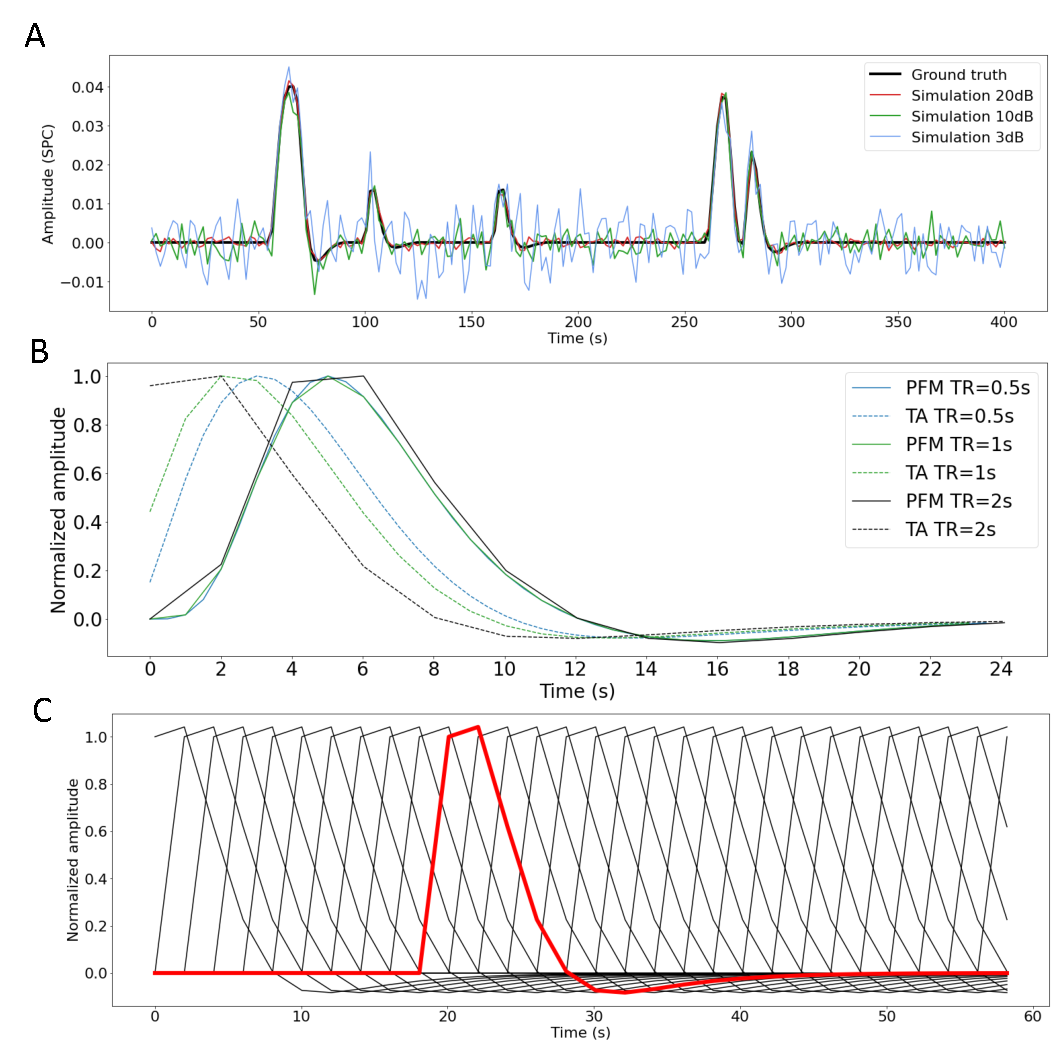
\includegraphics[width=\columnwidth]{figures/sim_and_hrf.pdf}
    \end{center}
    \caption{A) Simulated signal with different SNRs (20 dB, 10 dB and 3 dB) and ground truth. B) Canonical HRF models typically used by PFM (green) and TA (black) at TR = 0.1 s (dashed lines) and TR = 2 s (solid lines). Without loss of generality, the waveforms are scaled to unit amplitude for visualization. C) Representation of shifted HRFs at TR = 2 s that build the design matrix for PFM when the HRF model has been matched to that in TA. The red line corresponds to one of the columns of the HRF matrix.}
\label{fig:sim_and_hrf}
\end{figure}

%%%%%%%%%%%%%%%%%%%%%%%%%%%%%%%%%%%%%%%%%%%%%%%%%%%%%%%%%%%
%%%%%%%%%%%%%%%%%%%%%%%%%%%%%%%%%%%%%%%%%%%%%%%%%%%%%%%%%%%
%%%%%%%%%%%%%%%%%%%%%%%%%%%%%%%%%%%%%%%%%%%%%%%%%%%%%%%%%%%
\subsection{Experimental data}
\textbf{Motor task dataset:} One healthy subject was scanned in a 3T MR scanner (Siemens) as part of a larger experiment under a Basque Center on Cognition, Brain and Language Review Board-approved protocol. T2*-weighted multi-echo fMRI data was acquired with a multiband (MB) multi-echo gradient echo-planar imaging sequence (340 scans, 52 slices, Partial-Fourier = 6/8, voxel size = 2.4x2.4x3 mm\textsuperscript{3}, TR = 1.5 s, TEs = 10.6/28.69/46.78/64.87/82.96 ms, multiband factor = 4, flip angle = 70\(^o\), GRAPPA = 2).

During the fMRI acquisition, subjects performed a motor task consisting of five different movements (left-hand finger tapping, right-hand finger tapping, moving the left toes, moving the right toes and moving the tongue). These conditions were randomly intermixed every 16 seconds, and were only repeated once the entire set of stimuli were presented. Data preprocessing consisted of optimally combining the echo time datasets, detrending of up to 5\(^{th}\)-order Legendre polynomials, spatial smoothing (3 mm FWHM) and normalization to signal percentage change. The onset and duration of the different conditions can be seen in Figure~\ref{fig:task_maps}, along with the time-series of a representative voxel in the motor areas corresponding to each of the conditions.

\textbf{Resting-state datasets:} One healthy subject was scanned in a 3T MR scanner (Siemens) as part of a larger experiment under a Basque Center on Cognition, Brain and Language Review Board-approved protocol. Two runs of T2*-weighted fMRI data were acquired during resting-state, each with 10 min duration, with 1) a standard gradient-echo echo-planar imaging sequence (monoband) (TR = 2000 ms, TE = 29 ms, flip-angle = 78\(^o\), matrix size = 64x64, voxel size = 3x3x3 mm\textsuperscript{3}, 33 axial slices with interleaved acquisition, slice gap = 0.6 mm) and 2) a simultaneous multislice gradient-echo echo-planar imaging sequence (multiband factor = 3) developed by the Center of Magnetic Resonance Research (University of Minnesota, USA; TR = 800 ms, TE = 29 ms, flip-angle = 60\(^o\), matrix size = 64×64, voxel size = 3x3x3 mm\textsuperscript{3}, 42 axial slices with interleaved acquisition, no slice gap). Single-band reference images were also collected in both resting-state acquisitions for head motion realignment. Field maps were also obtained to correct for field distortions.

During both acquisitions, participants were instructed to keep their eyes open, fixating a white cross that they saw through a mirror located on the head coil, and not think about anything specific. The data was pre-processed using AFNI (\citealt{cox1996afni}). First, volumes corresponding to the initial 10 seconds were removed to allow for a steady-state magnetization. Then, the voxel time-series were despiked to reduce large-amplitude deviations and slice-time corrected. Inhomogeneities caused by magnetic susceptibility were corrected with FUGUE (FSL) using the field map images (\citealt{jenkinson2012fsl}). Next, functional images were realigned to a base volume (monoband: volume with the lowest head motion; multiband: single-band reference image). Finally, a simultaneous nuisance regression step was performed comprising up to 6th-order Legendre polynomials, low-pass filtering with a cutoff frequency of 0.25 Hz (only on multiband data to match the frequency content of the monoband), 6 realignment parameters plus temporal derivatives, 5 principal components of white matter (WM), 5 principal components of lateral ventricle voxels (anatomical CompCor) and 5 principal components of the brain's edge voxels. WM, CSF and brain's edge-voxel masks were obtained from Freesurfer tissue and brain segmentations. In addition, scans with potential artifacts were identified and censored as the euclidean norm of the temporal derivative of the realignment parameters (ENORM) was larger than 0.4, and the proportion of voxels adjusted in the despiking step exceeded 10\%.

%%%%%%%%%%%%%%%%%%%%%%%%%%%%%%%%%%%%%%%%%%%%%%%%%%%%%%%%%%%
%%%%%%%%%%%%%%%%%%%%%%%%%%%%%%%%%%%%%%%%%%%%%%%%%%%%%%%%%%%
%%%%%%%%%%%%%%%%%%%%%%%%%%%%%%%%%%%%%%%%%%%%%%%%%%%%%%%%%%%
\subsection{Selection of the hemodynamic response function}

With the aim of making a fair comparison between both methods, we first compared their HRFs. Figure~\ref{fig:sim_and_hrf}B shows the difference in the HRF that PFM and TA use by default for TR = 0.1 s and TR = 2 s adjusted to peak amplitude of one; i.e., the canonical HRF and the HRF resulting from the linear differential operator. The most observable difference between the two HRFs is the time to peak: the HRF used by Total Activation does not begin at zero\todo{But that's not related to TTP} while the one used by PFM does.

While PFM allows for the use of any HRF---the columns of the design matrix \(\mathbf{H}\) are composed by shifted versions of the HRF--- the linear differential operator in TA is tailored for a fixed HRF\todo{It's maybe not so simple: what I take from Elad's paper is that any convolution operator $\mathbf{H}$ (for synthesis) can be turned in an equivalent analysis operator.}. Hence, for practical reasons, we reproduced the HRF in the Total Activation filter and incorporated it into the PFM formulation (Figure~\ref{fig:sim_and_hrf}C).

%%%%%%%%%%%%%%%%%%%%%%%%%%%%%%%%%%%%%%%%%%%%%%%%%%%%%%%%%%%
%%%%%%%%%%%%%%%%%%%%%%%%%%%%%%%%%%%%%%%%%%%%%%%%%%%%%%%%%%%
%%%%%%%%%%%%%%%%%%%%%%%%%%%%%%%%%%%%%%%%%%%%%%%%%%%%%%%%%%%
\subsection{Selection of the regularization parameter}

Here, we use the simulated data to compare the performance of the two deconvolution algorithms with both selection criteria for the regularization parameter $\lambda$: a selection based on the BIC solution, and a selection based on the MAD estimate of the noise (see section \ref{sec:regparam}). We also evaluate if the algorithms behave differently in terms of the estimation of the activity-inducing signal $\mathbf{\hat{s}}$ using the \textit{spike model} in~\eqref{eq:pfm_spike} and the innovation signal $\mathbf{\hat{u}}$ using the \textit{block model} in~\eqref{eq:pfm_block}.

In order to calculate the regularization paths, we perform LARS with the PFM deconvolution model and obtain the solution for every $\lambda$ in the regularization path. Then, we use the values of $\lambda$ obtained with LARS to solve the TA deconvolution model by means of FISTA.

On the other hand, to solve the deconvolution problem with a selection based on the MAD estimate of the noise with PFM, we selected the $\lambda$ corresponding to the residuals that were closest to the estimated noise level of the data $\tilde{\sigma}$. We applied TA with temporal regularization in its original form and we do not introduce additional spatial regularization.

%%%%%%%%%%%%%%%%%%%%%%%%%%%%%%%%%%%%%%%%%%%%%%%%%%%%%%%%%%%
%%%%%%%%%%%%%%%%%%%%%%%%%%%%%%%%%%%%%%%%%%%%%%%%%%%%%%%%%%%
%%%%%%%%%%%%%%%%%%%%%%%%%%%%%%%%%%%%%%%%%%%%%%%%%%%%%%%%%%%
\subsection{Differences in experimental data}

In order to describe the extent of the discrepancies between the techniques, we calculate the sum of squares of the differences (SSD) between the estimated activity-inducing signals of PFM and TA on the three experimental datasets as:
\begin{equation}
    SSD = \frac{\sum_{k}{(\hat{s}_\text{PFM}[k] - \hat{s}_\text{TA}[k])^2}}{N},
\end{equation}
where $N$ is the number of frames of the acquisition. The SSD of the innovation signals $\mathbf{\hat{u}}$ was computed equally.

At the same time, we evaluate the performance of PFM and TA in comparison with a GLM that takes advantage of the duration and onsets of the stimuli in the motor task data. Given the block design of the motor task, we only make this comparison with the block model.

%%%%%%%%%%%%%%%%%%%%%%%%%%%%%%%%%%%%%%%%%%%%%%%%%%%%%%%%%%%
%%%%%%%%%%%%%%%%%%%%%%%%%%%%%%%%%%%%%%%%%%%%%%%%%%%%%%%%%%%
%%%%%%%%%%%%%%%%%%%%%%%%%%%%%%%%%%%%%%%%%%%%%%%%%%%%%%%%%%%
\subsection{Beyond deconvolution}
Finally, we show the usefulness of deconvolution approaches by using the activity-inducing and innovation signals obtained and performing a co-activation patterns (CAPs) and innovation-driven co-activation patterns (iCAPs) analysis. We calculate the average time-series in a seed of 9 voxels located in the precuneus, supramarginal gyrus and occipital gyri independently, and solve the deconvolution problem to find the activity-inducing and innovation signals in the seeds. We then average the maps of time-frames with an amplitude over the 95th percentile threshold and compare the results with the maps obtained by applying the same procedure to the original signal in the seed.